%%%%%%%%%%%%%%%%%%%%%%%%%%%%%%%%%%%%%%%%%
% Masters/Doctoral Thesis 
% LaTeX Template
% Version 2.5 (27/8/17)
%
% This template was downloaded from:
% http://www.LaTeXTemplates.com
%
% Version 2.x major modifications by:
% Vel (vel@latextemplates.com)
%
% This template is based on a template by:
% Steve Gunn (http://users.ecs.soton.ac.uk/srg/softwaretools/document/templates/)
% Sunil Patel (http://www.sunilpatel.co.uk/thesis-template/)
%
% Template license:
% CC BY-NC-SA 3.0 (http://creativecommons.org/licenses/by-nc-sa/3.0/)
%
%%%%%%%%%%%%%%%%%%%%%%%%%%%%%%%%%%%%%%%%%

%----------------------------------------------------------------------------------------
%	PACKAGES AND OTHER DOCUMENT CONFIGURATIONS
%----------------------------------------------------------------------------------------

\documentclass[
11pt, % The default document font size, options: 10pt, 11pt, 12pt
oneside, % Two side (alternating margins) for binding by default, uncomment to switch to one side
english, % ngerman for German
doublespacing, % Single line spacing, alternatives: onehalfspacing or doublespacing
%draft, % Uncomment to enable draft mode (no pictures, no links, overfull hboxes indicated)
nolistspacing, % If the document is onehalfspacing or doublespacing, uncomment this to set spacing in lists to single
%liststotoc, % Uncomment to add the list of figures/tables/etc to the table of contents
%toctotoc, % Uncomment to add the main table of contents to the table of contents
%parskip, % Uncomment to add space between paragraphs
%nohyperref, % Uncomment to not load the hyperref package
headsepline, % Uncomment to get a line under the header
%chapterinoneline, % Uncomment to place the chapter title next to the number on one line
%consistentlayout, % Uncomment to change the layout of the declaration, abstract and acknowledgements pages to match the default layout
]{MastersDoctoralThesis} % The class file specifying the document structure

\usepackage[utf8]{inputenc} % Required for inputting international characters
\usepackage[T1]{fontenc} % Output font encoding for international characters

\usepackage{mathpazo} % Use the Palatino font by default

\usepackage[backend=bibtex,style=ieee,natbib=true]{biblatex} % Use the bibtex backend with the authoryear citation style (which resembles APA)

\addbibresource{bib.bib} % The filename of the bibliography

\usepackage[autostyle=true]{csquotes} % Required to generate language-dependent quotes in the bibliography

%----------------------------------------------------------------------------------------
%	MARGIN SETTINGS
%----------------------------------------------------------------------------------------

\geometry{
	paper=a4paper, % Change to letterpaper for US letter
	inner=2.5cm, % Inner margin
	outer=3.8cm, % Outer margin
	bindingoffset=.5cm, % Binding offset
	top=1.5cm, % Top margin
	bottom=1.5cm, % Bottom margin
	%showframe, % Uncomment to show how the type block is set on the page
}

%----------------------------------------------------------------------------------------
%	THESIS INFORMATION
%----------------------------------------------------------------------------------------

\thesistitle{Efficient, Movement-Based Skeleton Action Recognition} % Your thesis title, this is used in the title and abstract, print it elsewhere with \ttitle
\supervisor{Dr. Robert \textsc{Laganière}} % Your supervisor's name, this is used in the title page, print it elsewhere with \supname
\examiner{} % Your examiner's name, this is not currently used anywhere in the template, print it elsewhere with \examname
\degree{Master of Computer Science, Specialization in Applied AI} % Your degree name, this is used in the title page and abstract, print it elsewhere with \degreename
\author{Nicolas \textsc{Fleece}} % Your name, this is used in the title page and abstract, print it elsewhere with \authorname
\addresses{} % Your address, this is not currently used anywhere in the template, print it elsewhere with \addressname

\subject{Computer Science} % Your subject area, this is not currently used anywhere in the template, print it elsewhere with \subjectname
\keywords{} % Keywords for your thesis, this is not currently used anywhere in the template, print it elsewhere with \keywordnames
\university{\href{http://www.university.com}{University of Ottawa}} % Your university's name and URL, this is used in the title page and abstract, print it elsewhere with \univname
\department{\href{http://department.university.com}{School of Electrical Engineering and Computer Science}} % Your department's name and URL, this is used in the title page and abstract, print it elsewhere with \deptname
\group{\href{http://researchgroup.university.com}{VIVA Research Lab}} % Your research group's name and URL, this is used in the title page, print it elsewhere with \groupname
\faculty{\href{http://faculty.university.com}{Faculty of Engineering}} % Your faculty's name and URL, this is used in the title page and abstract, print it elsewhere with \facname

\AtBeginDocument{
\hypersetup{pdftitle=\ttitle} % Set the PDF's title to your title
\hypersetup{pdfauthor=\authorname} % Set the PDF's author to your name
\hypersetup{pdfkeywords=\keywordnames} % Set the PDF's keywords to your keywords
}

\begin{document}

\frontmatter % Use roman page numbering style (i, ii, iii, iv...) for the pre-content pages

\pagestyle{plain} % Default to the plain heading style until the thesis style is called for the body content

%----------------------------------------------------------------------------------------
%	TITLE PAGE
%----------------------------------------------------------------------------------------

\begin{titlepage}
\begin{center}

\vspace*{.06\textheight}
{\scshape\LARGE \univname\par}\vspace{1.5cm} % University name
\textsc{\Large Doctoral Thesis}\\[0.5cm] % Thesis type

\HRule \\[0.4cm] % Horizontal line
{\huge \bfseries \ttitle\par}\vspace{0.4cm} % Thesis title
\HRule \\[1.5cm] % Horizontal line
 
\begin{minipage}[t]{0.4\textwidth}
\begin{flushleft} \large
\emph{Author:}\\
\href{http://www.johnsmith.com}{\authorname} % Author name - remove the \href bracket to remove the link
\end{flushleft}
\end{minipage}
\begin{minipage}[t]{0.4\textwidth}
\begin{flushright} \large
\emph{Supervisor:} \\
\href{http://www.jamessmith.com}{\supname} % Supervisor name - remove the \href bracket to remove the link  
\end{flushright}
\end{minipage}\\[3cm]
 
\vfill

\large \textit{A thesis submitted in fulfillment of the requirements\\ for the degree of \degreename}\\[0.3cm] % University requirement text
\textit{in the}\\[0.4cm]
\groupname\\\deptname\\[2cm] % Research group name and department name
 
\vfill

{\large \today}\\[4cm] % Date
%\includegraphics{Logo} % University/department logo - uncomment to place it
 
\vfill
\end{center}
\end{titlepage}

%----------------------------------------------------------------------------------------
%	ABSTRACT PAGE
%----------------------------------------------------------------------------------------

\begin{abstract}
\addchaptertocentry{\abstractname} % Add the abstract to the table of contents
The Thesis Abstract is written here (and usually kept to just this page). The page is kept centered vertically so can expand into the blank space above the title too\ldots
\end{abstract}

%----------------------------------------------------------------------------------------
%	QUOTATION PAGE
%----------------------------------------------------------------------------------------

\vspace*{0.2\textheight}

\noindent\enquote{\itshape Thanks to my solid academic training, today I can write hundreds of words on virtually any topic without possessing a shred of information, which is how I got a good job in journalism.}\bigbreak

\hfill Dave Barry

%----------------------------------------------------------------------------------------
%	ACKNOWLEDGEMENTS
%----------------------------------------------------------------------------------------

\begin{acknowledgements}
\addchaptertocentry{\acknowledgementname} % Add the acknowledgements to the table of contents
The acknowledgments and the people to thank go here, don't forget to include your project advisor\ldots
\end{acknowledgements}

%----------------------------------------------------------------------------------------
%	LIST OF CONTENTS/FIGURES/TABLES PAGES
%----------------------------------------------------------------------------------------

\tableofcontents % Prints the main table of contents

\listoffigures % Prints the list of figures

\listoftables % Prints the list of tables

%----------------------------------------------------------------------------------------
%	ABBREVIATIONS
%----------------------------------------------------------------------------------------

\begin{abbreviations}{ll} % Include a list of abbreviations (a table of two columns)

\textbf{LAH} & \textbf{L}ist \textbf{A}bbreviations \textbf{H}ere\\
\textbf{WSF} & \textbf{W}hat (it) \textbf{S}tands \textbf{F}or\\

\end{abbreviations}

%----------------------------------------------------------------------------------------
%	THESIS CONTENT - CHAPTERS
%----------------------------------------------------------------------------------------

\mainmatter % Begin numeric (1,2,3...) page numbering

\pagestyle{thesis} % Return the page headers back to the "thesis" style

% Include the chapters of the thesis as separate files from the Chapters folder
% Uncomment the lines as you write the chapters

% Chapter Template

\chapter{Introduction} % Main chapter title

\label{Chapter1} % Change X to a consecutive number; for referencing this chapter elsewhere, use \ref{ChapterX}

People interact with their environment in unique and nuanced ways, and throughout our lives, humans have learned to identify and categorize the different actions that we perform.

\section{Action Recognition}

For humans, the problem of human action recognition is rather simple. We use past experiences throughout childhood and adult life to be able to pick out the various ways a person moves, and translate that into a familiar action that we have seen before. Combine that with objects that a person may be interacting with, and humans are remarkably good at discerning what actions other humans are involved in. However, as is with most things in the domain of computer vision, this ability does not translate well into the realm of artificial intelligence. The slightly different ways that people may perform these tasks add a layer of complexity that is difficult for a model to overcome.

\section{Applications}

\textbf{Security} is perhaps the most obvious example of action recognition usage. Security personnel are constantly on the lookout for suspicious individuals that may be of concern, or who are performing illegal actions. This can be as simple as trying to find those who are shoplifting in stores, where the CCTV footage can be used live to find those who are actively stealing from stores. It could also be something more complex, such as security checkpoints in airports, where screening officers are constantly watching for suspicious individuals. In this case, a system capable of analyzing the way every person acts and pointing out those who it sees as suspicious could greatly assist security personnel.

\textbf{Health care} is a slightly different, but nonetheless very interesting application of action recognition. A very large part of how action recognition can help those in the healthcare field is use in monitoring those who need around the clock care, primarily the elderly. If an elderly person chooses to live at home, the action recognition model may allow healthcare workers to, at a distance, manage many people and focus their attention on those who have been flagged by the model. This can often be done by very lightweight models \cite{Eldermonitoring}.

\textbf{Video summarization} is perhaps not directly related to action recognition, but rather the study of action recognition is a very useful part of video summarization. If you must summarize a video where the main subjects tend to be humans, a large part of figuring out what is going on in the video is figuring out what action the person is performing, for example, for a summary to be something such as '\textit{The person is fishing.}', the model must have some understanding of what fishing is. Similarly, if the main subject of the video is not a person, it may still be useful to know what those in the background are doing, for example '\textit{A dog is sitting on a bench, there are people doing yoga in the background}', the model again must have an idea of what yoga is, and how a person performs said actions.

\subsection{Ethical Issues}

As with most applications of artificial intelligence, computer vision cannot be researched and discussed without taking into account the ethical issues that surround it. With AI being such a quickly evolving space, it is crucial that any researchers be aware of these issues. In this section, I will focus particularly on how it may affect action recognition, touching on other areas of AI in general to further illustrate my points.

\textbf{Privacy} can become a concern in many areas, the healthcare example given previously in this chapter is one of the most obvious. With elderly people, often one of the draws to staying in their own homes is the privacy that it offers; if the action recognition model is to be used to ensure that they remain safe, it must come with some removal of privacy. There is also a question of what happens to the data of a person who is using this kind of service. Since the data is almost certainly sent to a server to be processed, what kind of data retention policies might this company have in place, are they sharing this data with others, or is the data going to be used to train future models. These are all issues that often follow AI since the training of models requires such a massive amount of data, and in action recognition this can contain people who are not necessarily aware of their data being used in such ways.

\textbf{Bias} is one of the most common ethical issues in AI. In artificial intelligence, and computing in general, the principle of "garbage in, garbage out", is commonly used to illustrate that if the inputs into a model are not of high quality, the outputs will not be of high quality. This can often be the case in datasets where say a group of people are not accurately represented, and while the model itself is not discriminatory, it will follow the data it has been given. For example, airport security has been scrutinized in the past for singling out individuals of particular races or who look a particular way. This may mean that if a model is being constructed that searches for people who may be flagged later in security, the majority of positive flags that were screened further would be of this group of people. The resulting dataset that is constructed would be biased against this group of people, therefore resulting in a similarly-biased model. This type of issue has been shown in many different areas, another example being speech recognition models used by voice assistants not being able to recognize particular accents as they were not represented in the original dataset. These kinds of reasons are why it is crucial for researchers to be aware of and study their datasets when it comes to human data to avoid these biases and ensure that their data is well balanced.

\textbf{Transparency} is a rather difficult, and often nearly impossible problem to solve with modern AI models. Given the fact that these models at minimum have millions of parameters that all contribute to the complex calculations towards the output, deciphering exactly how they work and make their decisions is difficult. These models are often depicted as black boxes, where the only context we are given is what is input into the model and what the model outputs, and nothing in between. In the cases of something such as an airport security checkpoint, the model may mark a person as acting suspicious in a line of passengers. The model is not able to specifically express what made the passenger appear suspicious, and it may even be incorrect in its assumptions. This means that the officer who is reviewing the flags set by the model has to make a decision that leads to one of two possible scenarios:

\begin{enumerate}
	\item The model is correct, but cannot communicate its exact reasoning with the officer, the officer does not see what the model sees and a potential threat is ignored
	\item The model is incorrect, but the officer thinks that he sees something, and a person who is not a threat is put through unnecessary security screening, and other potential threats may not be screened
\end{enumerate}

\section{Challenges}
\label{sec:challenges}

Human action recognition is a very difficult task that comes with many issues, some of which continue to be major challenges moving forward with very complex modern models.

\textbf{Backgrounds} are often not static in videos. Often they contain a lot of data that is ever changing and can contain other secondary subjects performing actions that may not be relevant to the subject that we are trying to determine the action of. While humans are very good at focusing on the person who is performing the action and ignoring things occurring in the background enough to not get confused, AI models do not have this inherent ability and often can get confused from background changes, and effectively must both identify the person and determine what action they are performing within the same model. This can be further worsened by any camera movement, resulting in both the subject moving throughout the frame as well as the background moving behind the subject.

\section{Problem Definition}

The problem of human action recognition is defined as taking a video of a person performing a particular action, and passing it through a model to determine the specified action the person is performing. Pose-based action recognition is the problem of performing this detection primarily using the skeleton data of the people in the frame.

\section{Contributions}

The primary contribution that this thesis provides is a novel intermediate representation that can be used in tandem with a simple CNN for use in the problem of human action recognition. This representation is designed such that it is invariant to: the global position of the person, the distance between the camera and the person, and any background information. This representation only utilizes the skeleton data of the person, specifically the joint angles of a person and how they change from one frame to another.

\section{Thesis Structure}

This thesis will begin by exploring the research relevant to action recognition in chapter \ref{LiteratureReview}. Next, a novel representation is proposed in chapter \ref{Methodology}, and the experiments and their results are detailed in chapter \ref{Experimentation}. Finally, the conclusions and recommendations for future work are presented in chapter \ref{Conclusion}.
% Chapter Template

\chapter{Convolutional Neural Networks} % Main chapter title

\label{Chapter2} % Change X to a consecutive number; for referencing this chapter elsewhere, use \ref{ChapterX}

\section{Structure}

\section{Kernel Dimensions}

\subsection{3 Dimensional Convolutions}

\section{Classic Architectures}

\subsection{AlexNet}
\label{sec:alexnet}

\section{Modern Architectures}

\section{LSTMs}
\label{sec:LSTM} 
% Chapter Template

\chapter{Literature Review} % Main chapter title

\label{Chapter3} % Change X to a consecutive number; for referencing this chapter elsewhere, use \ref{ChapterX}

%Typical examples of action recognition \cite{i3d} have used complex convolutional neural networks (CNNs) on the RGB frames, pulling features such as rgb flow \cite{rgbflow} in order to enhance results. This method has proved to work well, however these models often require large amounts of GPU memory and are required to be run on high end hardware, which is a potential issue when applied to real-world scenarios where the necessary hardware may not be available. In addition, background noise is much more difficult to filter out and generalizing to different environments is difficult.

%A subset of action recognition models utilize skeleton-based action recognition. These models aim to utilize the positions of joints/bones in the model in order to filter out background data, and allow the model to focus on the actual person rather than background data. Typically these involve simpler CNNs that allow for faster computation on lower quality hardware. Many different approaches are used to achieve this action recognition. \cite{potion}, \cite{PA3D} utilize processed joint heatmap images and simple 2D-CNNs. \cite{simple_yet_efficient} \cite{smaller_faster_better} use intermediate representations to construct custom image representations that can be easily processed by simple CNNs. RNNs and LSTMs \cite{two_branch_stacked_lstm} \cite{RNN_joint_relative_motion} \cite{RNN_occlusion} \cite{DS_lstm} and Transformers \cite{transformersnippets} \cite{transformertwobranch} have been used as well to obtain good results with skeleton data.

%Almost always, these skeleton based models utilize 2D pose data. There have been some examples of extracting 3D pose from depth cameras \cite{depthcamera3dpose} as well as estimating 3D pose from 2D pose \cite{3dposefrom2d} and only the RGB frames \cite{2dposefromrgb}. These techniques have been used in the past for human action recognition \cite{3dposeactionrecognition}, however 2D pose estimation is a much easier task and the models that have been used are generally much higher quality, and therefore is more reliable for the task of human action recognition.

%----------------------------------------------------------------------------------------
%	Image Classification
%----------------------------------------------------------------------------------------
\section{Image Classification}

%----------------------------------------------------------------------------------------
%	Optical Flow
%----------------------------------------------------------------------------------------
\section{Optical Flow}

%----------------------------------------------------------------------------------------
%	CNN Models
%----------------------------------------------------------------------------------------
\section{CNN Based Models}

Naturally, the first approach to feeding video data into models is to process the raw RGB frames. The RGB frame data quite often 

%----------------------------------------------------------------------------------------
%	CNN + LSTM
%----------------------------------------------------------------------------------------
\subsection{CNN + LSTM Models}

The success of CNN's in the world of image classification makes the move to apply the same type of logic towards action recognition and the larger domain of video processing. Since a video broken down is just individual frames, the logic follows that we would be able to extract features from individual frames and combine these features to produce a classification outcome.

In very classic models, this is a very simple process. The individual frames are passed through the CNN model, producing a feature map for each frame. These feature maps are then simply pooled and passed into dense layers which produces an output. While very simple and fast, this model completely ignores any temporal activity, meaning that the model cannot determine how a person moves throughout a video from one frame to another. This would make differentiating some reversible actions such as running forwards vs running backwards.

Figure \ref{fig:cnn-lstm} shows the typical modern structure for this solution. After the features are extracted from each of the 2 dimensional CNN, they are passed through a LSTM. The goal of this LSTM module is to carry features from one frame to another.

\begin{figure}[t]
	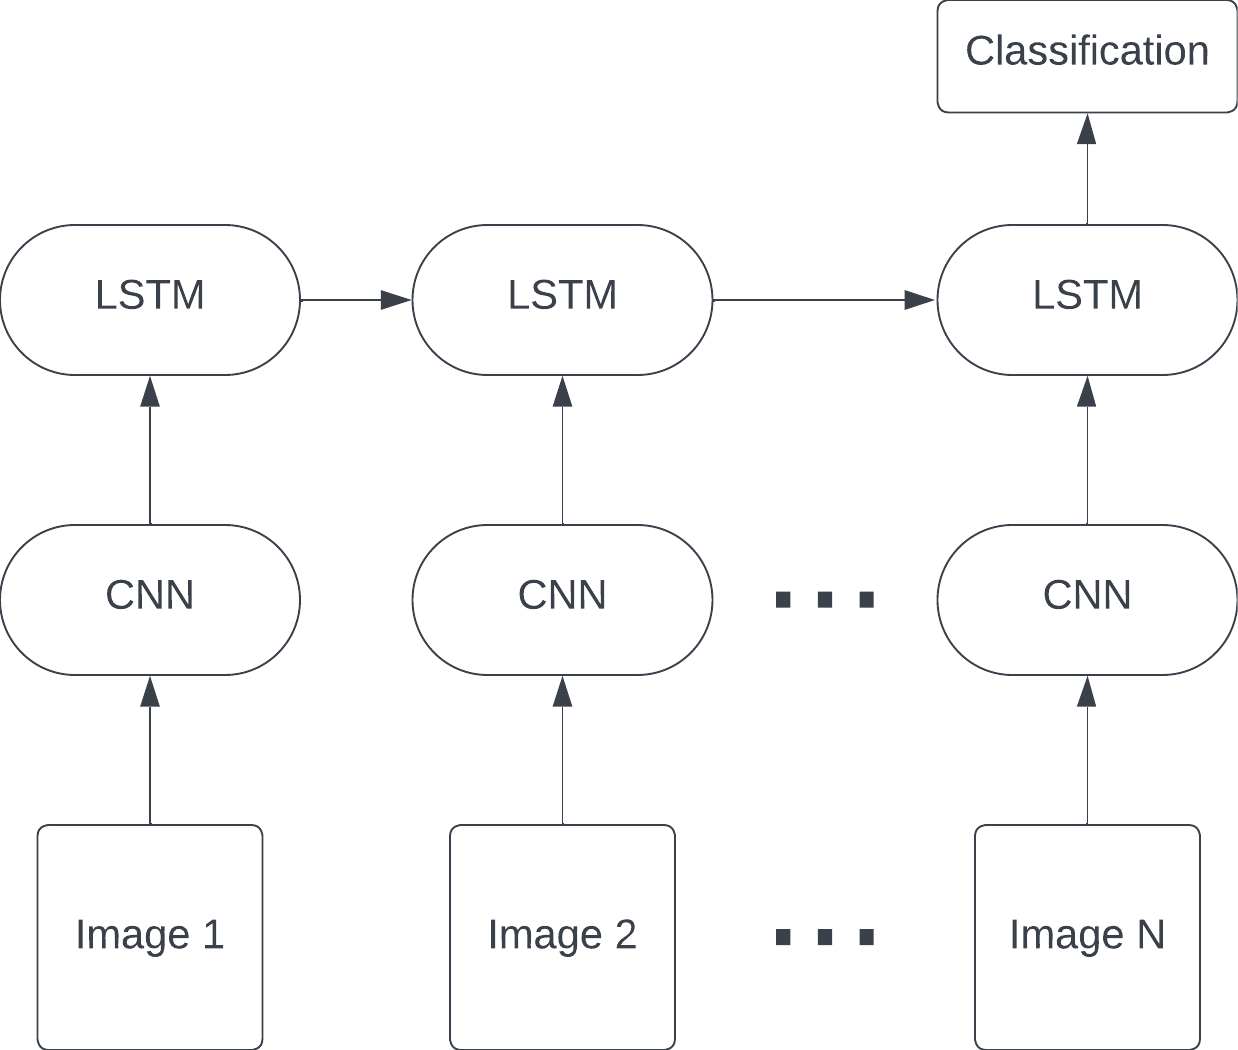
\includegraphics[width=8cm]{CNN-LSTM.png}
	\centering
	\caption{An example structure of a simple CNN-LSTM based model, each individual frame being individually fed into the CNN, and then passed to a LSTM.}
	\label{fig:cnn-lstm}
\end{figure}

The advantages of this model are that is is very lightweight and all of the individual parts are already well studied and efficient. This also means that the models are very lightweight, and relatively simple in comparison to more complex techniques.

The disadvantages of the model are also rooted in it's simplicity. The result of processing each image independently means that the interactions between frames is not very well represented. While the model is able to represent individual frame features very well, due to the fact that the feature maps are passed through the LSTM, classes that require specific movement from one frame to another are difficult to represent using this structure. Constructing these individual feature maps can also fall victim to background interference, meaning that a movement in the camera, or change in background could impact in a way that detracts from the main subject of the action more with this model than the other approaches discussed later in this chapter.

\begin{figure}[t]
	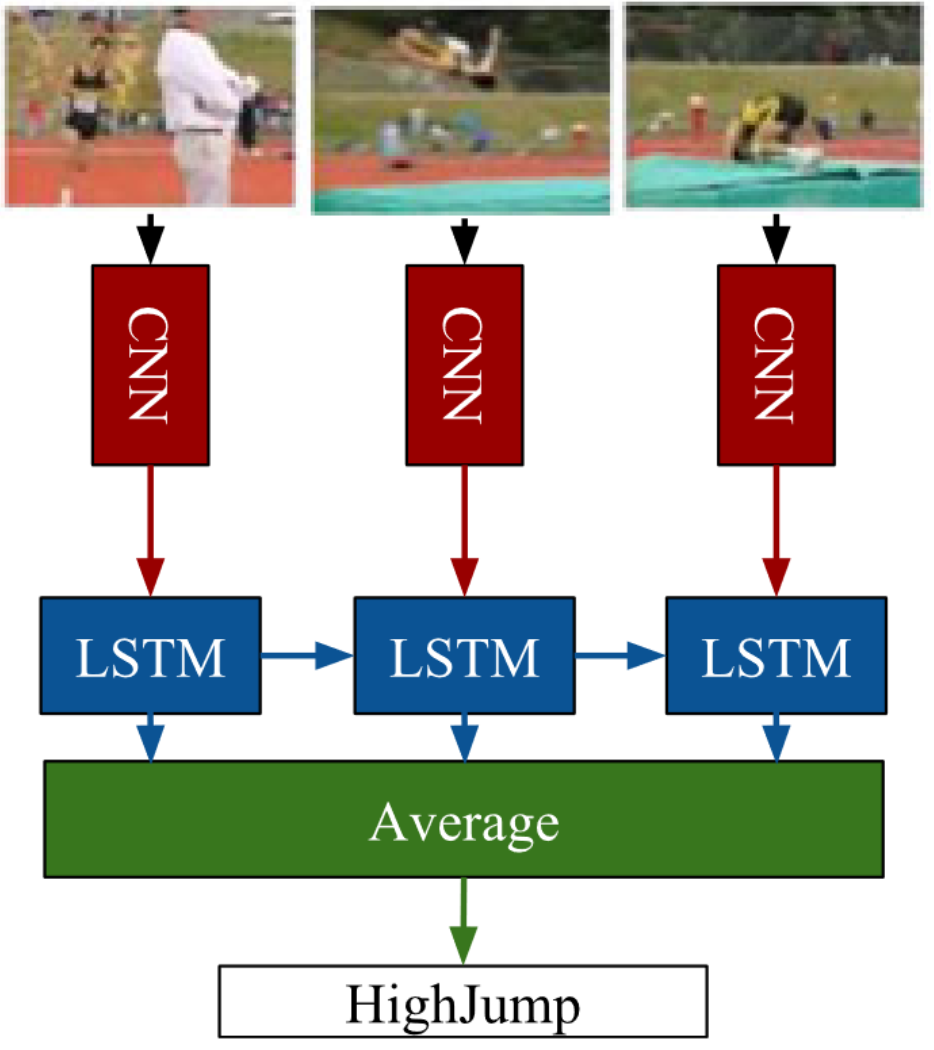
\includegraphics[width=8cm]{LRCN-AR.png}
	\centering
	\caption{Action recognition structure for the LRCN model. \cite{LRCNS}}
	\label{fig:lrcn-ar}
\end{figure}

\textbf{Long-term Recurrent Convolutional Networks} \cite{LRCNS}, is a model constructed using this methodology. In the paper, they use the notation that each frame, $x_{i}$, is fed into the CNN in order to construct a fixed-length feature representation, $\phi_{v}(x_{i})$. This is then passed into the recurrent sequence learning model. This is where the model differs from the previous example provided. In the LRCN model, the LSTM outputs at each frame are averaged to get the output class, rather than taking the last output. This removes any bias the model may have towards the later frames in long videos. In addition to RGB frames, this model additonally uses the optical flow feature, which easily adapts to this structure, replacing the RGB frames in figure \ref{fig:lrcn-ar}. The LSTM structure is taken from \cite{LSTM-2015}, which is a structure devised from the original LSTM model, as we discussed in section \ref{sec:LSTM}. The CNN's, represented in the paper as $\phi$, is described as a hybrid of the CaffeNet \cite{caffenet} (a variant of the AlexNet \cite{alexnet} model discussed in section \ref{sec:alexnet}) and the Zeiler and Fergus \cite{zeilerfergus} models, which has been pre-trained on a large dataset.

\begin{figure}[t]
	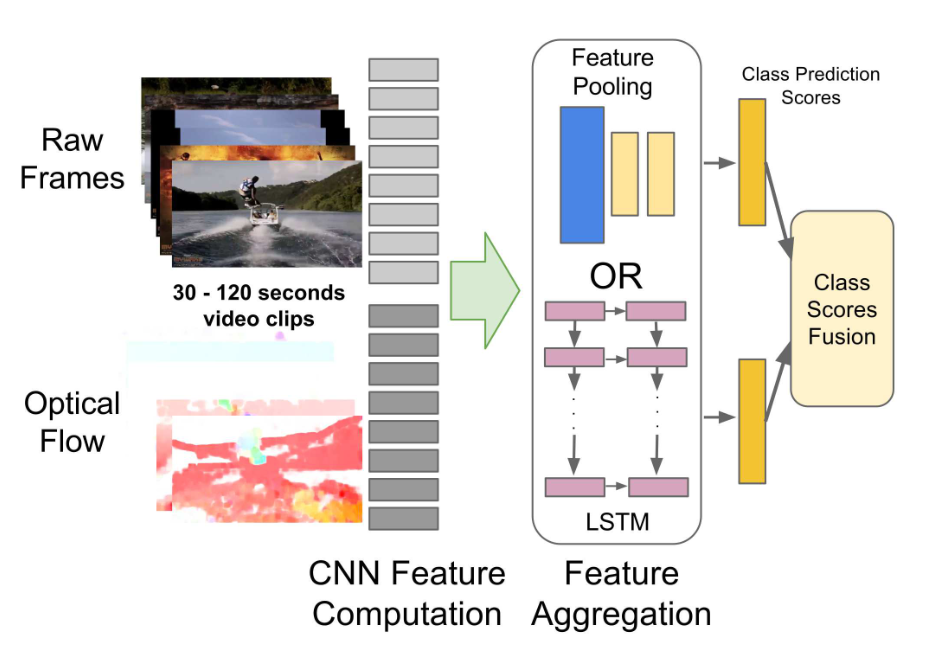
\includegraphics[width=10cm]{BeyondOverview.png}
	\centering
	\caption{Overview of the Beyond Short Snippets: Deep Networks for Video Classification model \cite{beyondshortsnippets}}
	\label{fig:beyondoverview}
\end{figure}

\textbf{Beyond Short Snippets: Deep Networks for Video Classification} \cite{beyondshortsnippets}, is another approach to this structure, which explores a more complex deep-LSTM based module, as well as more classical feature pooling. Similarly to the previously discussed model, Long-term Recurrent Convolutional Networks \cite{LRCNS}, the model utilizes a combination of two popular CNN models, AlexNet \cite{alexnet} and GoogLeNet \cite{googlenet}. The paper did explore many more classical feature pooling architectures, and were proven to have good results, however these techniques were outperformed by the LSTM model. The paper utilized a deep LSTM architecture for the feature aggregation step, shown in figure \ref{fig:deeplstm}, which further adds to it's complexity, moving it above the CNN-LSTM architectures described previously. In this deep-LSTM module, the outputs of each frame are passed into a LSTM module as in the previous model, but the ouputs are then passed up through 4 more stacked layers of LSTM's, after reaching softmax layers which are averaged to get an output. These 4 additional layers of LSTM's mean it is more able to infer data moving from one frame to another. This model additionally explored the uses of optical flow and found that it adds a great deal to the accuracy of the model.

\begin{figure}[t]
	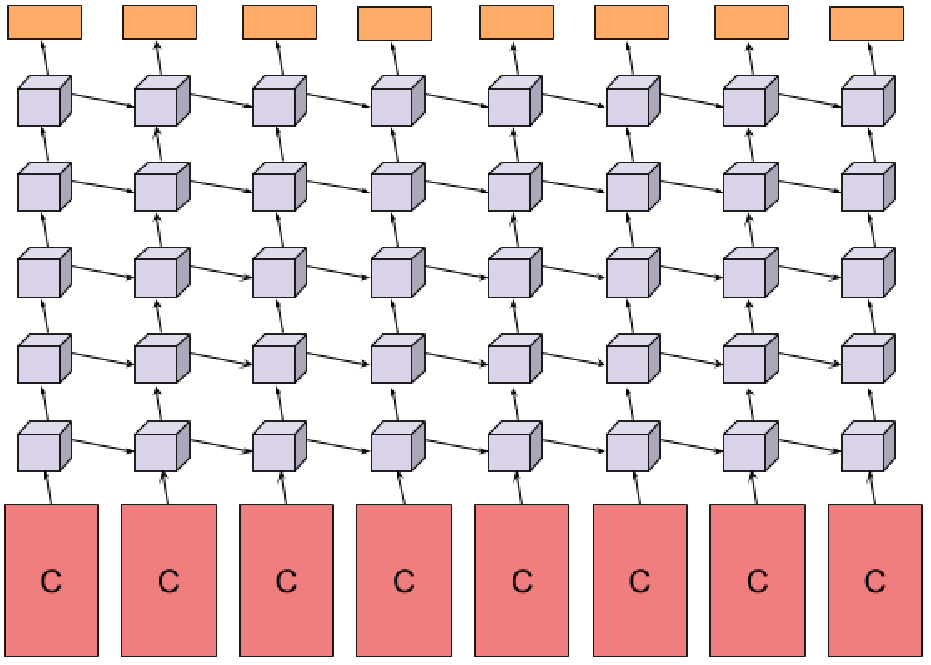
\includegraphics[width=8cm]{deepLSTM.png}
	\centering
	\caption{Deep LSTM architecture utilized by \cite{beyondshortsnippets} in the feature aggregation step as shown in figure \ref{fig:beyondoverview}.}
	\label{fig:deeplstm}
\end{figure}

%----------------------------------------------------------------------------------------
%	3D CNN
%----------------------------------------------------------------------------------------
\subsection{3D CNN Models}

When considering how to handle videos without the LSTM component, the most natural approach is to utilize 3 dimensional CNN kernels, the specifics of which were described in section \ref{3dkernels}. The function of these kernels when it relates to action recognition is that they allow for the model to easily encode local temporal data using the third kernel dimension. The primary issue with these models is that they contain many more parameters over the 2D CNN models, meaning that they take longer to train and require more computing power as compared to the lightweight counterparts.

\textbf{3D Convolutional Neural Networks for Human Action Recognition} \cite{3DCNN-ActionRecognition} was the original paper that proposed this model for the purposes of action recognition.

%----------------------------------------------------------------------------------------
%	Modern
%----------------------------------------------------------------------------------------
\section{Modern Methods}

%----------------------------------------------------------------------------------------
%	Datasets
%----------------------------------------------------------------------------------------
\section{Datasets}

%----------------------------------------------------------------------------------------
%	Skeleton Based Models
%----------------------------------------------------------------------------------------
\section{Skeleton-Based Action Recognition}

\subsection{Pose Detection}

\subsection{Intermediate Representations}
%% Chapter Template

\chapter{Methodology} % Main chapter title

\label{Methodology} % Change X to a consecutive number; for referencing this chapter elsewhere, use \ref{ChapterX}
 
%% Chapter Template

\chapter{Experimentation} % Main chapter title

\label{Experimentation} % Change X to a consecutive number; for referencing this chapter elsewhere, use \ref{ChapterX}

\section{Model Hyperparameters}

\subsection{Compute Resources}

\section{JHMDB Results}

\begin{table}[h]
	\centering
	\begin{tabular}{||c c||} 
		\hline
		\textbf{Split} & \textbf{Accuracy} \\ [0.5ex] 
		\hline\hline
		1 & 58.209\% \\ 
		\hline
		2 & 58.889\% \\
		\hline
		3 & 58.113\% \\
		\hline
		\hline
		\textbf{Average} & \textbf{58.404\%} \\
		\hline
	\end{tabular}
	\label{tab:acc-results}
	\caption{Results on all 3 splits of the JHMDB dataset utilizing only our novel approach.}
\end{table}

\begin{figure}[h]
	\includegraphics[width=10cm]{detailedPrecision}
	\centering
	\caption{Detailed precision results on the JHMDB dataset, averaged over the 3 testing splits. Black bars show the corresponding maximum \& minimum values attained in one of the splits.}
	\label{fig:detailed-precision}
\end{figure}

\begin{figure}[h]
	\includegraphics[width=10cm]{detailedRecall}
	\centering
	\caption{Detailed recall results on the JHMDB dataset, averaged over the 3 testing splits. Black bars show the corresponding maximum \& minimum values attained in one of the splits.}
	\label{fig:detailed-recall}
\end{figure}

\begin{figure}[h]
	\includegraphics[width=10cm]{detailedF1}
	\centering
	\caption{Detailed F1 score results on the JHMDB dataset, averaged over the 3 testing splits. Black bars show the corresponding maximum \& minimum values attained in one of the splits.}
	\label{fig:detailed-f1}
\end{figure}

\section{Model Ablation Study}

\begin{table}[h]
	\centering
	\begin{tabular}{||c c c||} 
		\hline
		\textbf{Split} & \textbf{Stacked} & \textbf{Only Angle Velocity} \\ [0.5ex] 
		\hline\hline
		1 & \textbf{58.209\%} & 48.888\% \\ 
		\hline
		2 & \textbf{58.889\%} & 44.444\% \\
		\hline
		3 & \textbf{58.113\%} & 41.132\% \\
		\hline
		\hline
		\textbf{Average} & \textbf{58.404\%} & 44.821\% \\
		\hline
	\end{tabular}
	\label{tab:acc-results-v-velocity}
	\caption{Comparison of results using only angle velocities vs the stacked representation.}
\end{table}

\begin{table}[h]
	\centering
	\begin{tabular}{||c c c||} 
		\hline
		\textbf{Split} & \textbf{Stacked} & \textbf{Only Angles} \\ [0.5ex] 
		\hline\hline
		1 & \textbf{58.209\%} & 56.343\% \\ 
		\hline
		2 & \textbf{58.889\%} & \textbf{58.889\%} \\
		\hline
		3 & \textbf{58.113\%} & 56.604\% \\
		\hline
		\hline
		\textbf{Average} & \textbf{58.404\%} & 57.279\% \\
		\hline
	\end{tabular}
	\label{tab:acc-results-v-angle}
	\caption{Comparison of results using only angles vs the stacked representation.}
\end{table}

\section{Model Comparison}
%% Chapter Template

\chapter{Conclusion \& Future Work} % Main chapter title

\label{Conclusion}

In this thesis, we have provided a novel representation for use in action recognition. This novel representation is unique to many other models in that it is invariant to:

\begin{itemize}
	\item Scale
	\item Global Position
\end{itemize}

We explore many different variations of this representation, concluding that the best representation contains both joint angle data and joint angle velocity data. It was also found that this data functions the best as a single image, with one data source stacked on top of another. This means that the combining of the angles and velocities can be learned by the convolutions slowly over the entire model, rather than typical fusion-like architectures that concatenate the different sources at the end.

With this representation, we were able to leverage a simple CNN model that is trainable on lightweight GPU's and is able to be tested on even lighter hardware. Despite the model being relatively lightweight, the model is able to provide 58.404\% average accuracy over the 3 splits of the JHMDB dataset. This shows that despite the model not having been fed any data about how the person is moving globally, or any data regarding the objects the person is interacting with, is able to fairly accurately predict what action the person is performing.

After further analyzing the results, the accuracy was shown to be slightly more nuanced than simply 58\% accurate overall. The model was able to predict classes that had more consistent movements that varied less from person to person such as golf or pullups, and tended to struggle with movements that can vary from person to person much more such as jump or catch.

\subsection{Future Work}

There is significant room for future work in this specific domain. Utilizing the skeleton data of a person to assist with action recognition is a constantly evolving domain, and has continually been proved to help existing models improve on their results. However, a perhaps more interesting area of research that is not quite as popular is intermediate representations, which is where the "low hanging fruit" are. The first place  of improvement would be to make the representation truly rotationally invariant, this would have to be done through a 3-dimensional pose detector, and modifications of how changes in rotations are represented in the end image. 

Another path forward is to more fully examine how real-time pose detection algorithms can be integrated with this simple model in order to obtain very fast and real-time results. This real-time computation is becoming more and more relevant in the world of smartphones, and examining how the model is able to be used on smartphones is crucial to determine the industrial applications. It is also worth noting that implementing this representation into existing complex models may be of interest in some applications, however the appeal of the representation being very lightweight and mobile applications not being as relevant cannot be ignored. 

%----------------------------------------------------------------------------------------
%	THESIS CONTENT - APPENDICES
%----------------------------------------------------------------------------------------

\appendix % Cue to tell LaTeX that the following "chapters" are Appendices

% Include the appendices of the thesis as separate files from the Appendices folder
% Uncomment the lines as you write the Appendices

% Appendix A

\chapter{Frequently Asked Questions} % Main appendix title

\label{AppendixA} % For referencing this appendix elsewhere, use \ref{AppendixA}

\section{How do I change the colors of links?}

The color of links can be changed to your liking using:

{\small\verb!\hypersetup{urlcolor=red}!}, or

{\small\verb!\hypersetup{citecolor=green}!}, or

{\small\verb!\hypersetup{allcolor=blue}!}.

\noindent If you want to completely hide the links, you can use:

{\small\verb!\hypersetup{allcolors=.}!}, or even better: 

{\small\verb!\hypersetup{hidelinks}!}.

\noindent If you want to have obvious links in the PDF but not the printed text, use:

{\small\verb!\hypersetup{colorlinks=false}!}.

%\include{Appendices/AppendixB}
%\include{Appendices/AppendixC}

%----------------------------------------------------------------------------------------
%	BIBLIOGRAPHY
%----------------------------------------------------------------------------------------

\printbibliography[heading=bibintoc]

%----------------------------------------------------------------------------------------

\end{document}  
